%----------------------------------------------------------------------------------------
%	PACKAGES AND THEMES
%----------------------------------------------------------------------------------------

\documentclass{beamer}

\mode<presentation> {
\usetheme{Madrid}
}

\usepackage{graphicx}
\usepackage{booktabs}
\usepackage{polski}
\usepackage[polish]{babel}
\usepackage[utf8]{inputenc}
\usepackage[T1]{fontenc}
\usepackage[utf8]{luainputenc}
\usepackage{pgfgantt}
\usepackage{caption}

% Strona tytułowa
\usepackage{pgfplots}
\usepackage{siunitx}
\usepackage{paracol}
\usepackage{gensymb}

% Pływające obrazki
\usepackage{float}
\usepackage{svg}
\usepackage{graphicx}


\DeclareCaptionFormat{citation}{%
   \ifx\captioncitation\relax\relax\else
     \captioncitation\par
   \fi
   #1#2#3\par}
\newcommand*\setcaptioncitation[1]{\def\captioncitation{\tiny{\textit{Źródło:}~#1}\medskip}\normalsize}
\let\captioncitation\relax
\captionsetup{format=citation,justification=centering}

\usetikzlibrary{pgfplots.groupplots}
\sisetup{detect-weight,exponent-product=\cdot,output-decimal-marker={,},per-mode=symbol,binary-units=true,range-phrase={-},range-units=single}

%wymiar tekstu
\def\figurename{Rys.}
\def\tablename{Tab.}

%----------------------------------------------------------------------------------------
%	TITLE PAGE
%----------------------------------------------------------------------------------------

\title[Seminarium Dyplomowe Inżynierskie]{Integracja części manipulacyjnej i bazy mobilnej robota Velma na potrzeby symulacji}

\author{Jakub Sikora} 
\institute[]
{
Zakład Sterowania Systemów \\
Instytut Automatyki i Informatyki Stosowanej \\
\medskip
Promotor: dr inż. Tomasz Winiarski
}
\date{13 grudnia 2019}

\AtBeginSection[]
{
    \begin{frame}[plain, noframenumbering]
        \frametitle{Agenda}
        \tableofcontents[currentsection]
    \end{frame}
}

\begin{document}

\begin{frame}
\titlepage
\end{frame}

\begin{frame}
\frametitle{Agenda}
\tableofcontents
\end{frame}

%----------------------------------------------------------------------------------------
%	PRESENTATION SLIDES
%----------------------------------------------------------------------------------------

\section{Cele pracy} 

\section{Przegląd istniejących symulatorów robota Velma} 

\begin{frame}
    \frametitle{Część manipulacyjna Velbody}
    \begin{figure}
        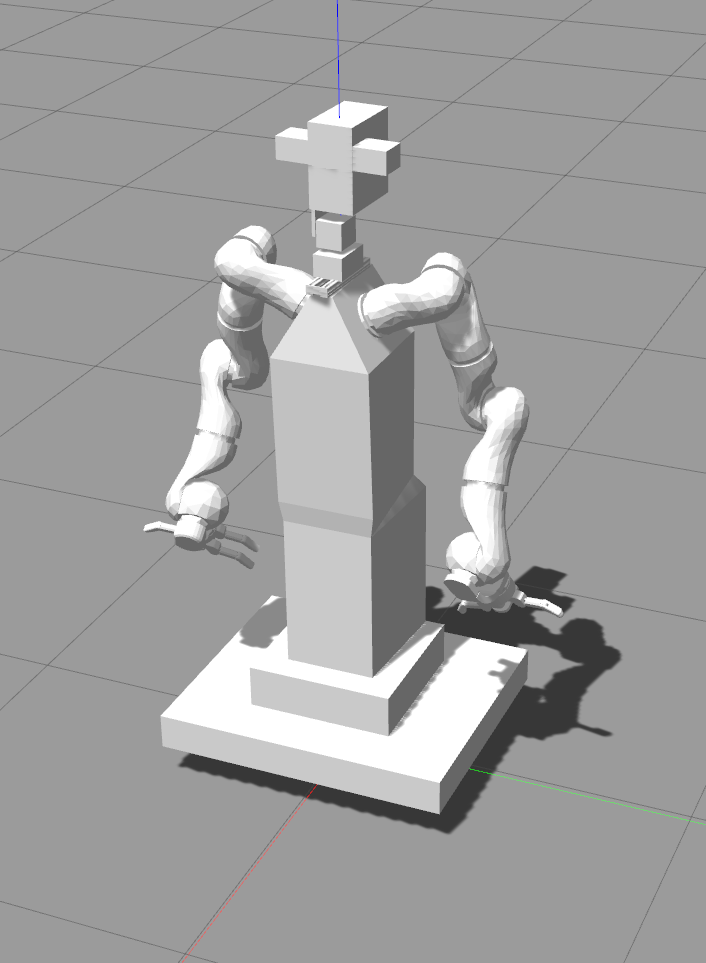
\includegraphics[scale=0.20]{./images/velma_gz_cropped.png}
        \caption{\normalsize{Część manipulacyjna robota Velma w symulatorze Gazebo}}
    \end{figure}
\end{frame}

\begin{frame}
    \frametitle{Część manipulacyjna Velbody}
    Część manipulacyjna robota Velma składa się z \cite{docsVelma}:  
    \begin{itemize}
        \item obrotowego korpusu
        \item dwóch manipulatorów KUKA LWR
        \item dwóch chwytaków BarrettHand
        \item szyi o dwóch stopniach swobody
        \item kamery Kinect XBOX 360
        \item czujników sił i momentu
        \item sztucznej skóry
        \item czujników Optoforce
    \end{itemize}
\end{frame}

\begin{frame} 
    \frametitle{Baza mobilna Velmobil}
    \begin{figure}
    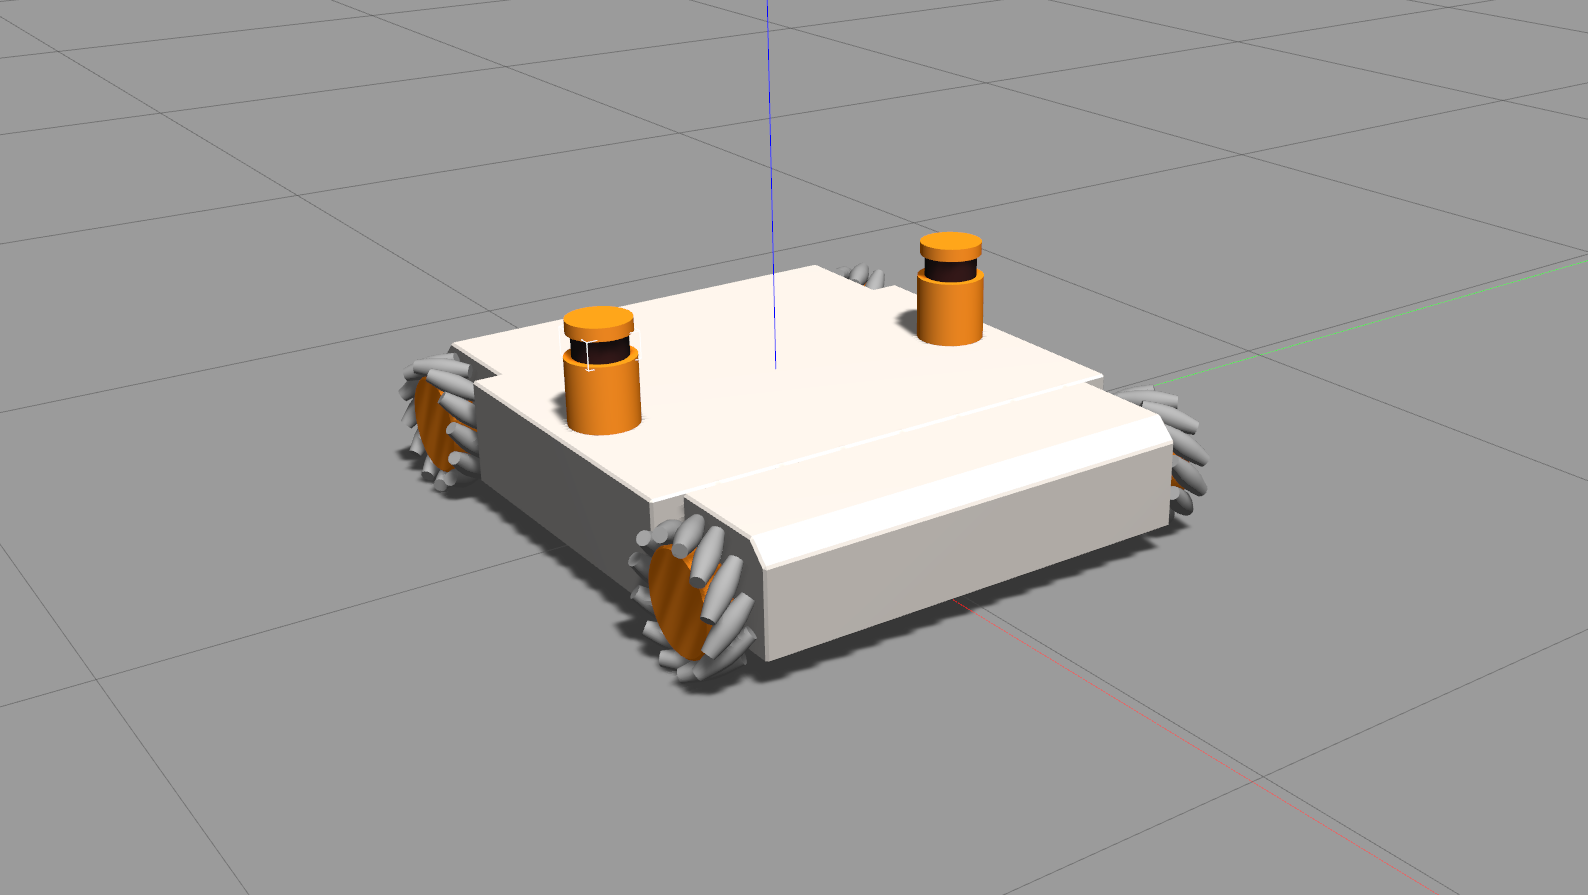
\includegraphics[scale=0.20]{./images/omnivelma_gz.png}
    \caption{Baza mobilna robota Velma w symulatorze Gazebo}
    \end{figure}
\end{frame}

\begin{frame}
    \frametitle{Baza mobilna Velmobil}
    Pojazd Velmobil posiada \cite{walas}:  
    \begin{itemize}
        \item 4 koła szwedzkie
        \item dwa skanery laserowe LIDAR
        \item jednostkę inercyjną
        \item enkodery % jakie enkodery
    \end{itemize}
\end{frame}
\section{Rozwiązanie problemu} 

\begin{frame}
    \frametitle{Integracja modeli symulacyjnych}
    \begin{figure}
        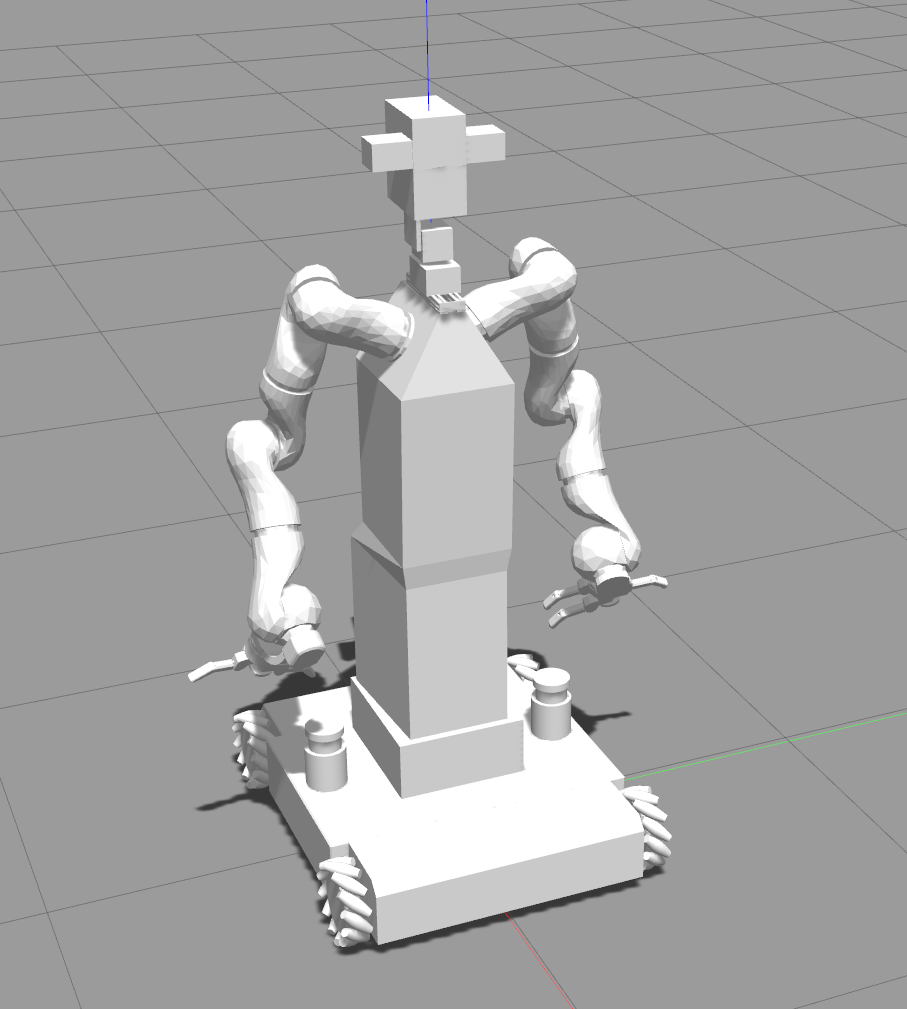
\includegraphics[scale=0.20]{./images/omnivelmobil-final-cropped.png}
        \caption{Zintegrowany robot Velma w symulatorze Gazebo}
    \end{figure}
\end{frame}

\begin{frame}
    \frametitle{Ogólna struktura projektowanego systemu} 
    \begin{figure}[b]
        \label{rosgraph_example}
        \centering
        \def\svgwidth{\columnwidth}
        \vspace{0.1cm}
        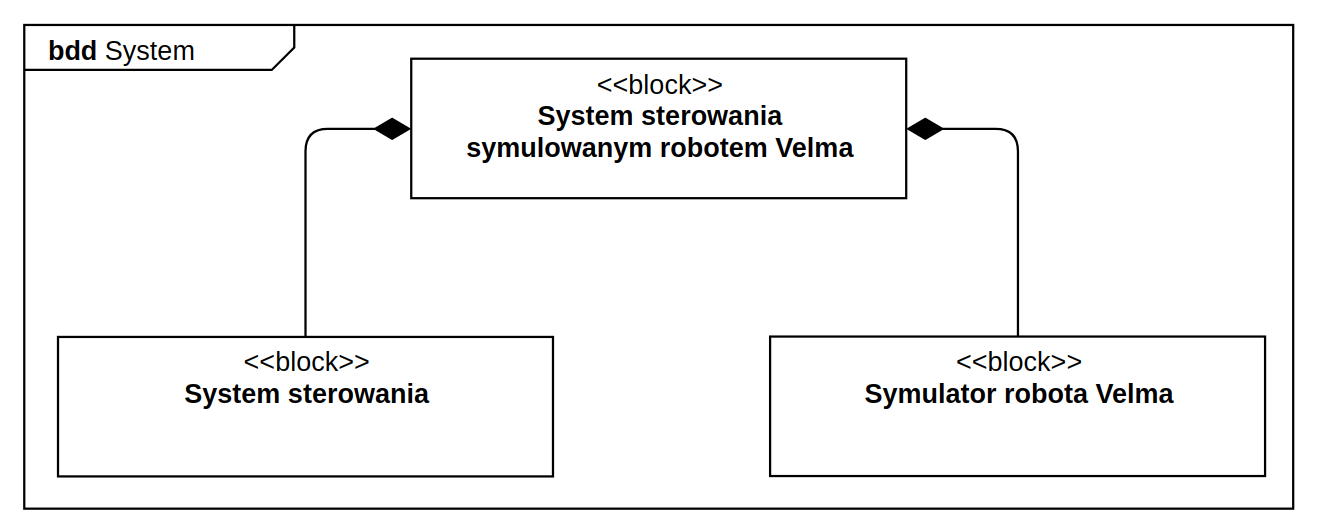
\includegraphics[scale=0.25]{images/basic_system.png}
        \vspace{0.1cm}
        \caption{Bazowa struktura projektowanego systemu}
    \end{figure}
\end{frame}

\begin{frame}
    \frametitle{Struktura symulatora robota Velma} 
    %% opis części symulacyjnej - podział na modele, silnik i wtyczki
\end{frame}

\begin{frame}
    \frametitle{Zasada działania kontrolera bazy mobilnej} 
    %% opis zmian które zaszły w kontrolerze bazy mobilnej po zmianie silnika fizyki
\end{frame}

\begin{frame}
    \frametitle{Struktura systemu sterowania} 
    %% opis systemu sterującego - opis sterowania częścią manipulacyjną i bazą mobilną
\end{frame}





\section{Wyniki badań} 

\begin{frame}
\frametitle{Badania regulatorów prędkości zadanej}
	\begin{figure}[t]
	    \centering
		 \begin{tikzpicture}
			\begin{axis}[
			width=0.95\textwidth,
			height=0.75\textheight,
			grid=major,
			xmin=0, xmax=37, ymin=0.0, ymax=0.5,
			xlabel={$t$},
			ylabel={$v(t)$},
			xtick={5, 10, 15, 20, 25, 30, 35},
			legend pos=north west,
			legend style={nodes={scale=0.6, transform shape}, font={\large}},
			legend image post style={mark=-}],
			y tick label style={/pgf/number format/1000 sep=},
			]
				\addplot[blue, semithick] file{ ./data/controllers/cmd_vel_linear_x.csv };
			    \addplot[red, semithick] file{ ./data/controllers/cmd_vel_linear_y.csv };
			    \addplot[green, semithick] file{ ./data/controllers/cmd_vel_angular_z.csv };
			    \addlegendentry{$v_{x}(t)$},
			    \addlegendentry{$v_{y}(t)$},
			    \addlegendentry{$\omega(t)$},
			    \addlegendimage{no markers, blue}
			    \addlegendimage{no markers, red}
				\addlegendimage{no markers, green}
			    \end{axis}
		    \end{tikzpicture}
		\caption{Trajektoria prędkości zadanej}
	\end{figure}
\end{frame}


\begin{frame}
\frametitle{Badania regulatorów prędkości zadanej}
	\begin{figure}[t]
	    \centering
		 \begin{tikzpicture}
			\begin{axis}[
			width=0.95\textwidth,
			height=0.75\textheight,
			grid=major,
			xmin=0, xmax=37, ymin=-0.1, ymax=0.3,
			xlabel={$t$},
			ylabel={$v(t)$},
			xtick={10, 20, 30, 40},
			legend pos=north west,
			legend style={nodes={scale=0.6, transform shape}, font={\large}},
			legend image post style={mark=-}],
			y tick label style={/pgf/number format/1000 sep=},
			]
				\addplot[blue, semithick] file{ ./data/controllers/odom_linear_x.csv };
			    \addplot[red, semithick] file{ ./data/controllers/cmd_vel_linear_x.csv };
			    \addlegendentry{$v_{\mathrm{zad}}(t)$},
			    \addlegendentry{$v(t)$},
			    \addlegendimage{no markers, red}
				\addlegendimage{no markers, blue}
			    \end{axis}
		    \end{tikzpicture}
		\caption{Porównanie przebiegów prędkości liniowej w osi x}
	\end{figure}
\end{frame}

\begin{frame}
\frametitle{Badania regulatorów prędkości zadanej}
	\begin{figure}[t]
	    \centering
		 \begin{tikzpicture}
			\begin{axis}[
			width=0.95\textwidth,
			height=0.75\textheight,
			grid=major,
			xmin=0, xmax=37, ymin=-0.1, ymax=0.3,
			xlabel={$t$},
			ylabel={$v(t)$},
			xtick={10, 20, 30, 40},
			legend pos=north west,
			legend style={nodes={scale=0.6, transform shape}, font={\large}},
			legend image post style={mark=-}],
			y tick label style={/pgf/number format/1000 sep=},
			]
				\addplot[blue, semithick] file{ ./data/controllers/odom_linear_y.csv };
			    \addplot[red, semithick] file{ ./data/controllers/cmd_vel_linear_y.csv };
			    \addlegendentry{$v_{\mathrm{zad}}(t)$},
			    \addlegendentry{$v(t)$},
			    \addlegendimage{no markers, red}
				\addlegendimage{no markers, blue}
			    \end{axis}
		    \end{tikzpicture}
		\caption{Porównanie przebiegów prędkości liniowej w osi y}
	\end{figure}
\end{frame}


\begin{frame}
\frametitle{Badania regulatorów prędkości zadanej}
	\begin{figure}[t]
	    \centering
		 \begin{tikzpicture}
			\begin{axis}[
			width=0.95\textwidth,
			height=0.75\textheight,
			grid=major,
			xmin=0, xmax=37, ymin=-0.3, ymax=0.6,
			xlabel={$t$},
			ylabel={$v(t)$},
			xtick={10, 20, 30, 40},
			legend pos=north west,
			legend style={nodes={scale=0.6, transform shape}, font={\large}},
			legend image post style={mark=-}],
			y tick label style={/pgf/number format/1000 sep=},
			]
				\addplot[blue, semithick] file{ ./data/controllers/odom_angular_z.csv };
			    \addplot[red, semithick] file{ ./data/controllers/cmd_vel_angular_z.csv };
			    \addlegendentry{$v_{\mathrm{zad}}(t)$},
			    \addlegendentry{$v(t)$},
			    \addlegendimage{no markers, red}
				\addlegendimage{no markers, blue}
			    \end{axis}
		    \end{tikzpicture}
		\caption{Porównanie przebiegów prędkości kątowej}
	\end{figure}
\end{frame}
%------------------------------------------------

\begin{frame}[plain]
\addtocounter{framenumber}{-1}
\frametitle{Bibliografia}
\footnotesize{
\begin{thebibliography}{99} % Beamer does not support BibTeX so references must be inserted manually as below
\bibitem[1]{docsVelma} D. Seredyński
\newblock Documentation of control system of WUT Velma Robot, 2017.
\newblock \url{https://rcprg-ros-pkg.github.io/velma\_docs/}.

\bibitem[2]{walas} P. Walas
\newblock Nawigacja robota mobilnego w bezpośrednim otoczeniu człowieka
\newblock \emph{Praca dyplomowa inżynierska}, Promotor: dr hab. inż. Wojciech Szynkiewicz, 2018.

\bibitem[3]{bezpieczenstwo} T.Winiarski
\newblock Wybrane aspekty bezpieczeństwa w badaniach robotów usługowych
\newblock \emph{Politechnika Warszawska}, materiały do Sterowania i Symulacji Robotów, 2018.

\bibitem[4]{sterowanie} T. Winiarski, C. Zieliński
\newblock Podstawy sterowania siłowego robotów
\newblock{Pomiary Automatyka Robotyka}, 6/2008, strony 5-10.

\end{thebibliography}
}
\end{frame}

%------------------------------------------------

\begin{frame}[plain]
\addtocounter{framenumber}{-1}
\Huge{\centerline{Dziękuję za uwagę}}
\end{frame}

%% dodatkowe
\addtocounter{framenumber}{-1}
\begin{frame}[plain]
    \frametitle{Przykładowy dodatkowy slajd}
\end{frame}

\end{document} 